\documentclass[a4paper]{article}

\usepackage[T1]{fontenc}
\usepackage[utf8]{inputenc}
\usepackage[english]{babel}
\usepackage{csquotes}
\usepackage{listings}
\usepackage{multicol}
\lstset{language=c,frame=single,captionpos=b}
\usepackage{hyperref}
\usepackage{amsmath}
\usepackage[backend=biber, sorting=none,maxbibnames=40]{biblatex}
\renewbibmacro{in:}{}
\addbibresource{ref.bib}
\usepackage{graphicx}
\usepackage{placeins}
\usepackage[margin=2.5cm]{geometry}
\usepackage{subcaption}
\usepackage[affil-it]{authblk}
\usepackage{color}
\usepackage{amssymb,amsmath}
\usepackage{subfloat}
\usepackage{float}

\begin{document}
\title{GPU Assignment: Image processing}
\author{Stefano Sandonà}
\affil{Vrije Universiteit Amsterdam, Holland}
\date{}
		
\maketitle

\section{GPUs: NVIDIA GTX480}
\label{sec:nvidia}
The aim of this assignment was to learn how to use many-core accelerators, GPUs in this particular case, to parallelize data-intensive code. All the implementations were written for the \textbf{NVIDIA GTX480}, using CUDA, a parallel computing platform and programming model invented by NVIDIA. Programming with CUDA, there is a straightforward mapping onto hardware, for this reason it is necessary to study the available HW before start developing an application. The architecture of the given accelerator is is shown in Figure \ref{fig:gtx}, its main characteristics and limits are shown in Table \ref{table:t1}.

\begin{figure}[ht]
    \centering
    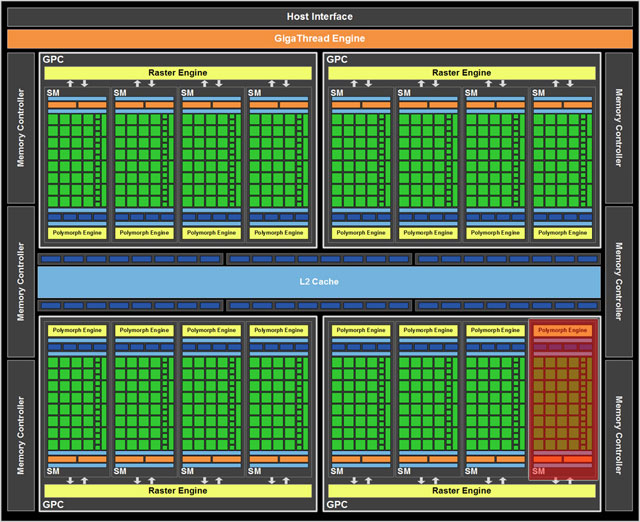
\includegraphics[width=0.7\linewidth]{gtx}
    \caption{NVIDIA GTX480 Architecture}
    \label{fig:gtx}
\end{figure}
\FloatBarrier

\begin{table}[ht]
\centering
\begin{tabular}{l|l}
Microarchitecture & Fermi \\ \hline
Compute capability (version) & 2.0 \\ \hline
Maximum dimensionality of grid of thread blocks & 3 \\ \hline
Maximum x-dimension of a grid of thread blocks & 65535 \\ \hline
Maximum y-, or z-dimension of a grid of thread blocks & 65535 \\ \hline
Maximum dimensionality of thread block & 3 \\ \hline
Maximum x- or y-dimension of a block & 1024 \\ \hline
Maximum number of threads per block & 1024 \\ \hline
Cores per SM (warp size) & 32 \\ \hline
SM & 15 \\ \hline
Cores & 480 (32 * 15) \\ \hline
Maximum number of resident blocks per multiprocessor & 8 \\ \hline
Maximum number of resident warps per multiprocessor & 48 \\ \hline
Maximum number of resident threads per multiprocessor & 1536 (48 * 32) \\ \hline
Number of 32-bit registers per multiprocessor & 32K \\ \hline
Maximum amount of shared memory per multiprocessor & 48K
\end{tabular}
\caption{NVIDIA GTX480 Specifications}
\label{table:t1}
\end{table}


\section{CImg}
\label{sec:cimg}
The image processing library used in this project was CImg, a small, modern and open-source toolkit developed for C++. CImg implements the RGB color model, an additive color model in which red, green, and blue light are added together in various ways to reproduce a broad array of colors. Each colored image of size \textit{N*M} is composed by three parts (R,G,B) of the same size, so that \textit{N*M*3} values are necessary to define an image. The Figure \ref{fig:rgb} shows an example of image composition.

\begin{figure}[ht]
    \centering
    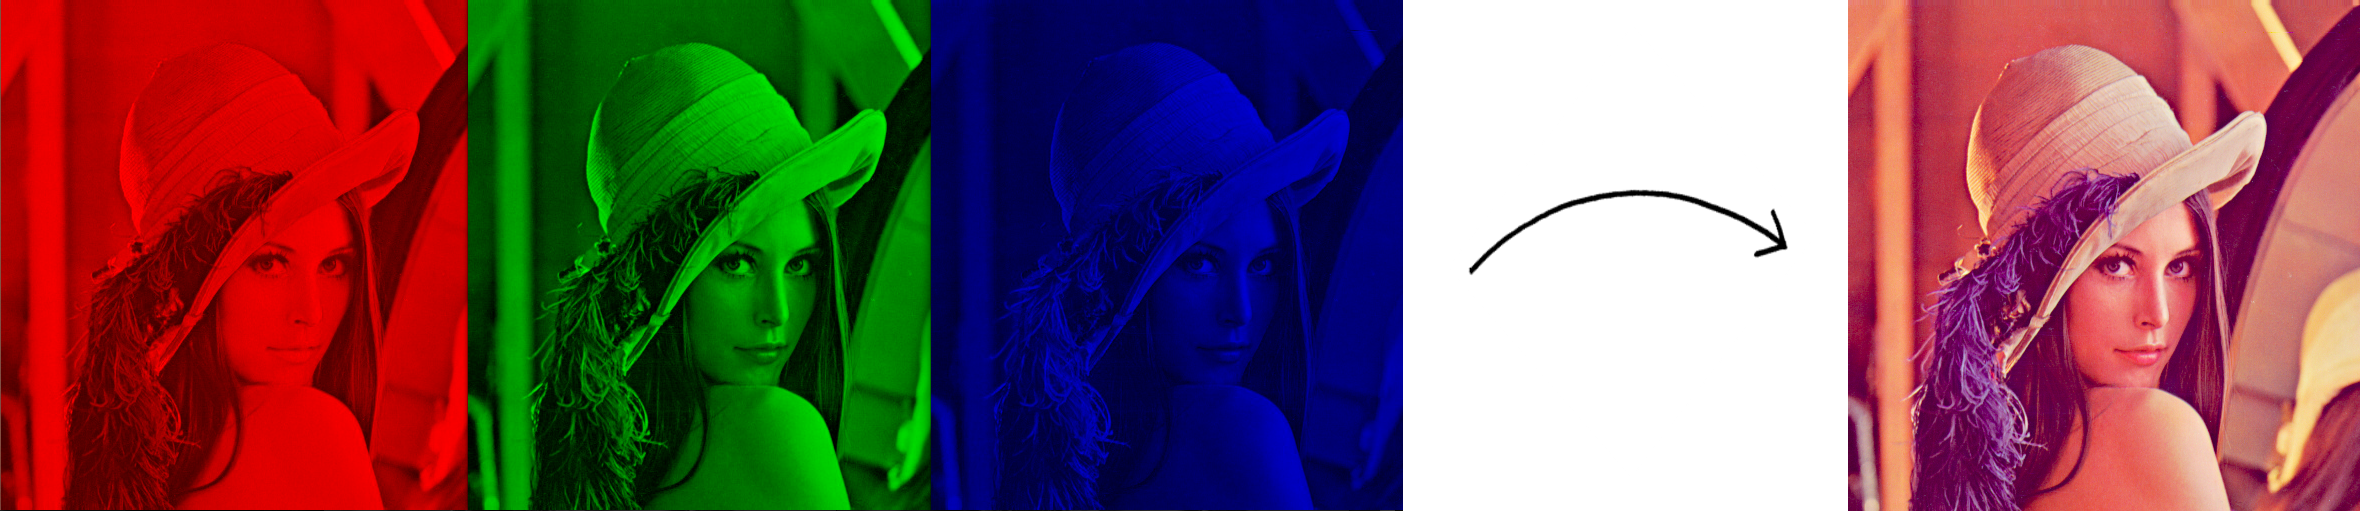
\includegraphics[width=0.7\linewidth]{rgb}
    \caption{RGB model}
    \label{fig:rgb}
\end{figure}
\FloatBarrier

\section{The processing flow}
\label{sec:cpf}
Using CUDA there are two parts of the code: the device code, or GPU code, or the Kernel, that is a sequential program, write for one thread and execute for all and the HOST code, or CPU code, that is used to instantiate the grid, run the kernel, manage the memory. Figure \ref{fig:flow} shows the processing flow of a CUDA application. In the particular case of image processig, everything starts from the CPU, that store the image from a file into a local buffer, allocates IN and OUT buffers on the GPU (\textit{cudaMalloc}) and copy the image into the GPU's IN buffer (\textit{cudaMemCpy}). After that, the CPU launches the GPU kernel with a defined grid configuration (\textit{kernel\_function <<gridDim, blockDim>>(params)}), that is executed by the GPU following the SIMT (Single Instruction, Multiple Threads) NVIDIA model. The threads are executed in parallel in each core, and they read the assigned part of IN data and generates the assigned part of OUT data. At the end, the results are copied out back to the CPU (\textit{cudaMemCpy}) and the image is written to a file by the CPU.

\begin{figure}[ht]
    \centering
    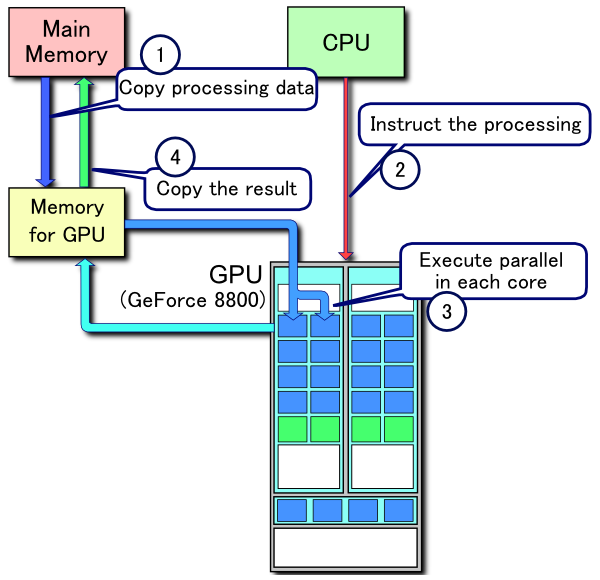
\includegraphics[width=0.5\linewidth]{flow}
    \caption{CUDA processing flow}
    \label{fig:flow}
\end{figure}
\FloatBarrier

\section{CUDA grid configuration}
\label{sec:grid}
In CUDA, as mentioned before, there is a strinct mapping with the hardware, so that an hardware virtualization model is fixed with the concepts of thread, block and grid.
Each \textbf{thread} executes the kernel code, running on one CUDA core.
The threads are logically grouped into \textbf{thread blocks}, so that the threads of the same block will run on the same multiprocessor. The thread blocks are logically organized in a \textbf{Grid}, that represent the entire dataset. The blocks and the grid can be of 1D, 2D or 3D.
An image is a 2D structure and for this reason the most convenient choice is to set up also a 2D grid. However, setting up a 2D grid, there is not only one way to follow. For this particular project, 4 possible combinations were considered. The first was a non square grid of 1D blocks (Figure \ref{fig:ns1}), the second a square grid with 1D blocks (Figure \ref{fig:s1}), the third a non square grid of 2D blocks (Figure \ref{fig:ns2}) and the third a square grid of 2D blocks (Figure \ref{fig:s2}). Different configurations were tested in order to find the best to suit the particular case.

\begin{figure}[!ht]
\begin{subfigure}{0.5\textwidth}
\centering
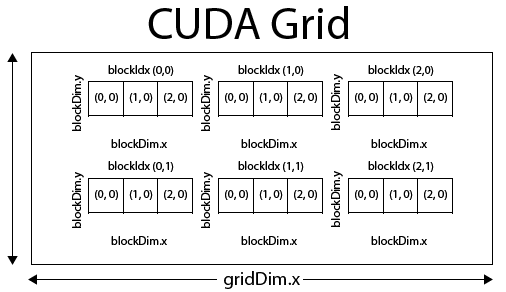
\includegraphics[width=\linewidth]{res/1D_no_square}
\caption{No square grid with 1D blocks}
\label{fig:ns1}
\end{subfigure} % separation between the subfigures
\begin{subfigure}{0.5\textwidth}
\centering
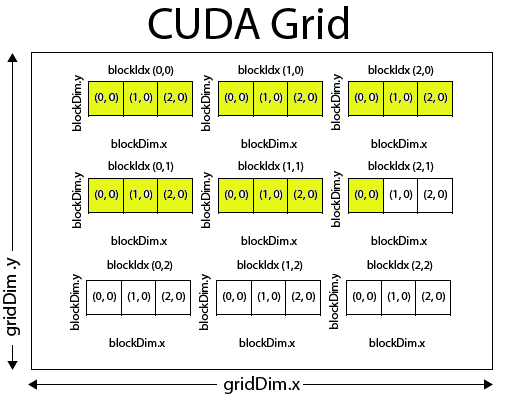
\includegraphics[width=\linewidth]{res/1D_square}
\caption{Square grid with 1D blocks}
\label{fig:s1}
\end{subfigure}
 % separation between the subfigures
\begin{subfigure}{0.5\textwidth}
\centering
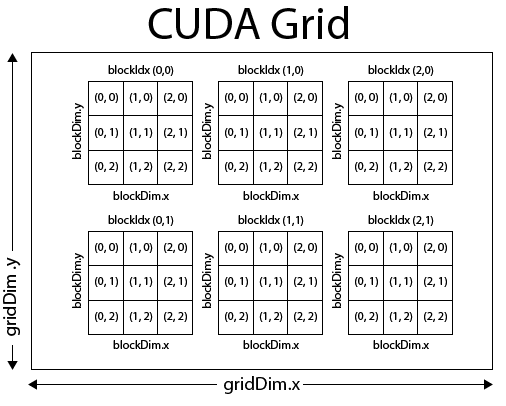
\includegraphics[width=\linewidth]{res/2D_no_square}
\caption{No square grid with 2D blocks}
\label{fig:ns2}
\end{subfigure}
 % separation between the subfigures
\begin{subfigure}{0.5\textwidth}
\centering
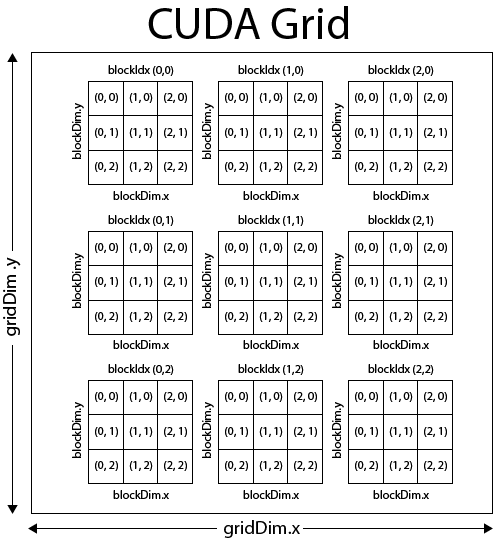
\includegraphics[width=\linewidth]{res/2D_square}
\caption{Square grid with 2D blocks}
\label{fig:s2}
\end{subfigure}
\caption{Possible kernel configurations}
 \label{fig:speed}
\end{figure}
\FloatBarrier

\section{Coalesced memory access}
\label{sec:cma}
One of the main bottlenecks with the GPUs is the global memory access that is expensive. CUDA uses a SIMT approach, in which all threads of a warp execute the same instruction. If the kernel is correctly designed, when the threads of a warp ask a value stored in the global memory, instead of having one access per thread, these accesses can be grouped if consecutive threads access consecutive memory addresses. This practise, is very useful to reduce the memory overhead, so that it was adopted in each algorithm.


\section{Algorithm 1: Grayscale Conversion and Darkening}
\label{sec:gcd}
From an RGB image, the output of this algorithm is a darker grayscale image.
The gray value of a pixel is generated by weighting the three values (\texttt{0.3*R, 0.59*G, 0.11*B}) and then summing them together. To darken the obtained grayscale image, the final pixel value is multiplied by a constant (0.6). The Figure \ref{fig:dark} shows an example of the result. The sequential algorithm, simply go through the entire image and computes for each pixel the corresponding value (Figure \ref{loop}).

\begin{figure}[ht]
    \centering
    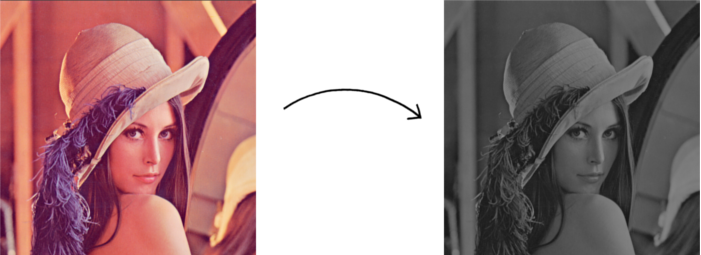
\includegraphics[width=\linewidth]{dark}
    \caption{Grayscale Conversion and Darkening}
    \label{fig:dark}
\end{figure}
\FloatBarrier

\begin{lstlisting}[label=loop, caption=Sequential code]
for ( int y = 0; y < height; y++ ) {
		for ( int x = 0; x < width; x++ ) {
			...
			float r = static_cast< float >(inputImage[(y * width) + x]);
			float g = static_cast< float >(inputImage[(width * height) + (y * width) + x]);
			float b = static_cast< float >(inputImage[(2 * width * height) + (y * width) + x]);
			...
			darkGrayImage[(y * width) + x] = static_cast< unsigned char >(grayPix);
\end{lstlisting}
\FloatBarrier

\subsection{Parallelization}
\label{sec:p1}
\subsection{First method}
\label{sec:fm}
After copying the input image into the GPU global memory and allocating some memory to content the output image, the kernel is ready to be launched. The GPU code is the same as the code content inside the loop of the sequential version (Figure \ref{loop}), but instead of using the indexes of the loop to access the image pixels, it uses the index associated to the thread. To exploit the coalesced memory access, two consecutive threads computes/accesses the values of two consecutive pixels. Different grid configurations were tested launching this program. 


M1=uni block overflow M2=uni block square M3=square block overflow M4=square block square
\begin{figure}[ht]
    \centering
    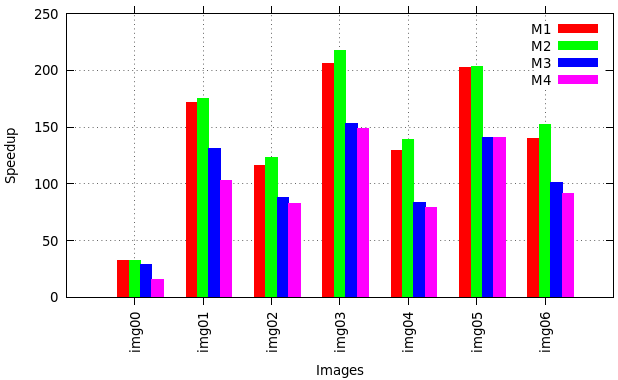
\includegraphics[width=0.9\linewidth]{res/darker_histo}
    \caption{Normalized Speedup}
    \label{fig:histo_darker}
\end{figure}
\FloatBarrier

Uni blocks, overflow (more) - M1 more
\begin{figure}[ht]
    \centering
    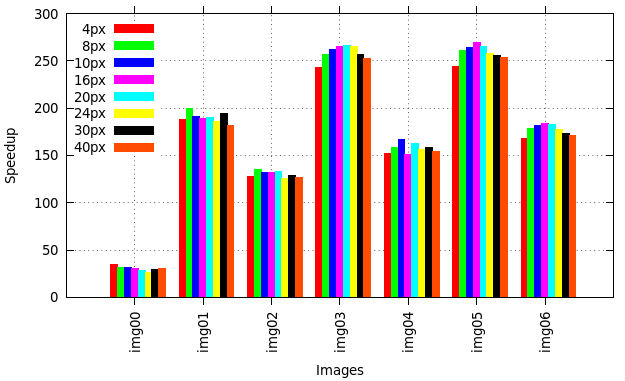
\includegraphics[width=0.9\linewidth]{res/darker_try_histo}
    \caption{Normalized Speedup}
    \label{fig:norm_histo_darker}
\end{figure}
\FloatBarrier

Uni blocks, square grid (more) - M2 more
\begin{figure}[ht]
    \centering
    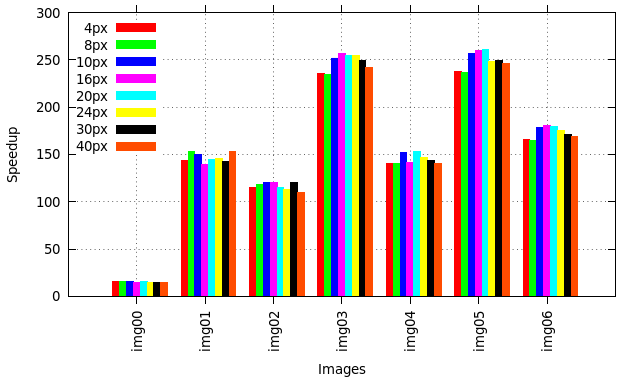
\includegraphics[width=0.9\linewidth]{res/darker_square_more_histo}
    \caption{Normalized Speedup}
    \label{fig:norm_histo_darker}
\end{figure}
\FloatBarrier

\begin{figure}[ht]
    \centering
    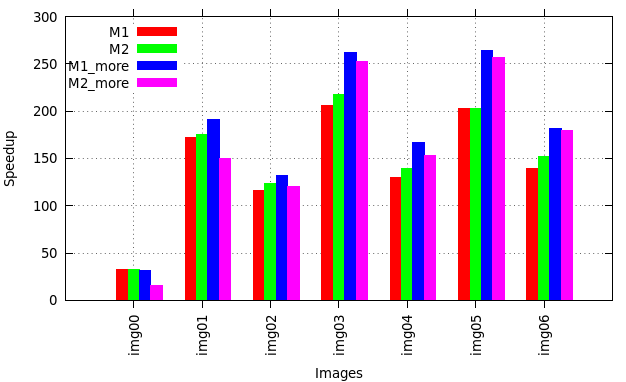
\includegraphics[width=0.9\linewidth]{res/darker_best_comparison}
    \caption{Normalized Speedup}
    \label{fig:norm_histo_darker}
\end{figure}
\FloatBarrier

\section{Algorithm 2: Histogram Computation}
\label{sec:hc}
From an RGB image, the output of this algorithm is a grayscale image with the relative histogram of 256 possible values of gray.
The histogram measures how often a value of gray is used in an image. The sequential algorithm, simply go through the entire image, computing for each pixel the corresponding gray value and incrementing the corresponding counter. The Figure \ref{fig:histo} shows an example of the result.

\begin{lstlisting}[label=loop2, caption=Sequential code]
for ( int y = 0; y < height; y++ ) {
		for ( int x = 0; x < width; x++ ) {
			float grayPix = 0.0f;
			float r = static_cast< float >(inputImage[(y * width) + x]);
			float g = static_cast< float >(inputImage[(width * height) + (y * width) + x]);
			float b = static_cast< float >(inputImage[(2 * width * height) + (y * width) + x]);

			grayPix = ((0.3f * r) + (0.59f * g) + (0.11f * b)) + 0.5f;

			grayImage[(y * width) + x] = static_cast< unsigned char >(grayPix);
			histogram[static_cast< unsigned int >(grayPix)] += 1;
		}
}
\end{lstlisting}

\begin{figure}[ht]
    \centering
    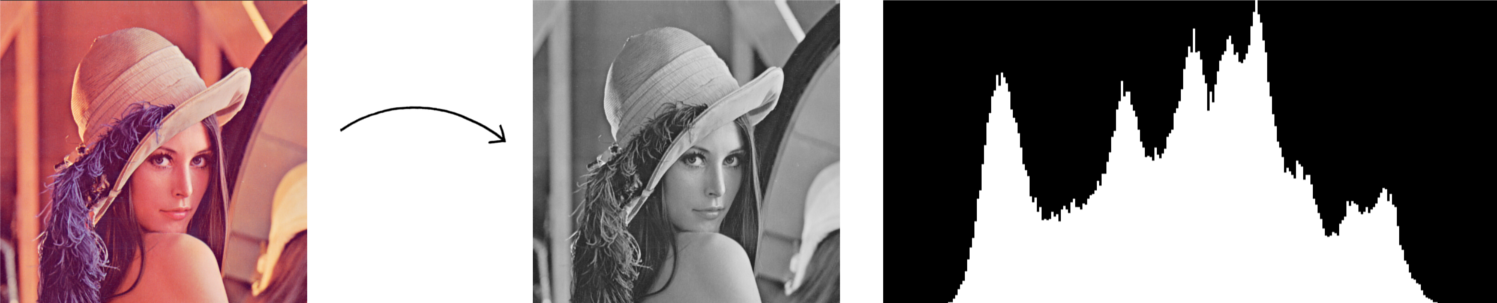
\includegraphics[width=0.7\linewidth]{histo}
    \caption{Histogram Computation}
    \label{fig:histo}
\end{figure}
\FloatBarrier

\subsection{Parallelization}
\label{sec:p2}
\subsection{First method}
\label{sec:fm2}
After copying the input image and the initial empty histogram into the GPU global memory and allocating some memory to content the output image, the kernel is ready to be launched. As for the previous algorithm, the GPU code is the same as the code content inside the loop of the sequential version (Figure \ref{loop2}), but instead of using the indexes of the loop to access the image pixels, it uses the index associated to the thread. Also in this case, to exploit the coalesced memory access, two consecutive threads computes/accesses the values of two consecutive pixels. The interesting aspect of the histograms, is that it is possible that two threads read at the same time read the same value of gray for a pixel, so that at the same time they try to increment the same corresponding histogram bin. For a correct execution, to avoid wrong updates, the increment has to be an atomic operation, so that only one thread at the time will modify the bin value. 

The logic behind an atomic operations is that each thread "locks" the variable, modify it, and "unlocks" it, so that the other threads that try to modify the same variable has to wait that this will be "unlocked". The worst case, in the histogram scenario, is a monocromo image, in which all the threads try to modify the same bin, which implies a long waiting queue of threads.
 Different grid configurations were tested launching this program. 


\section{Algorithm 3: Smoothing}
\label{sec:smoo}
Smoothing is the process of removing noise from an image by the means of statistical analysis. To remove the noise, each point is replaced by a weighted average of its neighbours. In this way small-scale structures are removed from the image. In this case a two-dimensional 5-point triangular smooth filter was used. The Figure \ref{fig:smooth} shows an example of the result.

\begin{figure}[ht]
    \centering
    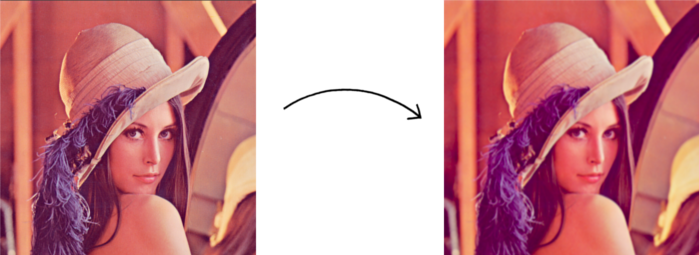
\includegraphics[width=0.5\linewidth]{smooth}
    \caption{Smoothing}
    \label{fig:smooth}
\end{figure}
\FloatBarrier

\subsection{Parallelization}
\label{sec:p2}
This particular algorithm deals with square areas of the image (filter), so that using 2D blocks, the threads can efficiently share memory and prevent a lot of global memory accesses.

\begin{figure}[!ht]
\begin{subfigure}{0.5\textwidth}
\centering
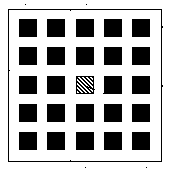
\includegraphics[width=\linewidth]{filter}
\caption{No square grid with 1D blocks}
\label{fig:ns1}
\end{subfigure} % separation between the subfigures
\begin{subfigure}{0.5\textwidth}
\centering
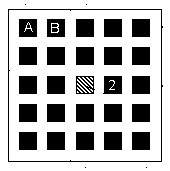
\includegraphics[width=\linewidth]{filter_letters}
\caption{Square grid with 1D blocks}
\label{fig:s1}
\end{subfigure}
\caption{Possible kernel configurations}
 \label{fig:speed}
\end{figure}
\FloatBarrier

\section{Algorithms analysis with the Visual Profiler}
\label{sec:vp}

\subsection{Application 1}
\label{sec:a1}
After collecting the profile of the applications using \textbf{nvprof}, the output files were evaluated using the \textbf{Nvidia Visual Profiler}.

\begin{lstlisting}[label=loop, caption=Sequential code]

float g = static_cast< float >(inputImage[(width * height) + (y * width) + x]);
float b = static_cast< float >(inputImage[(2 * width * height) + (y * width) + x]);

\end{lstlisting}
\FloatBarrier

For all the images the profiler found no issues for \textit{Divergent Execution} (threads that follow different if branches) and a \textit{Warp Execution Efficiency} (ratio of the average active threads per warp to the maximum number of threads per warp supported on a multiprocessor) of 100\%. This last value comes from the fact that is used a block of 256 threads, that is a multiple of 32 (warp size), so no useless threads are launched and from the fact that there is no thread divergent execution, so the threads within a warp can execute in a SIMD way, avoiding inactive threads within a warp. 

is defined as "." his will be low if you launch a non-multiple of 32 threads, if threads in a warp exit early, or if you have a divergent thread execution

 and Global Memory Access Pattern. All images, occupancy over 91\% except the first 82.5\%. Block size 256, 12 registers, 0 shared memory. Warp efficiency 
 


Blocks multiple of warps otherwise idle threads. Switching between concurrent warps (no overhead because registers and share memory are partitioned they are not stored/restored  to hide latency, if another warp is ready => switch, for this reason we need high number of warps or instruction level parallelism (2 dependents instruction, the second is waiting the output of a previous)

1)Exposing sufficient parallelism
HW more aritmetic throughput than memory bandwidth
Maximize the use of bytes that travel from DRAM to SM => memory accesses per warp, memory accessed in discrete chunks, threads in a warp provide 32 addresses, hw convert addresses into memory transactions (expensive), 
WRITE
a warp of threads consecutive and they fall in the same rigion (128bytes consecutives) => single memory transaction

On image number 5 => no coalesced access for the 2 instructions.. because image pixels non a multiple of 128, so non aligned (threadID+pizelsOfImage) but not effect the computation, compiling with -Xptxas -dlcm=cg worst results, Changing the configuration (cudaDeviceSetCacheConfig(cudaFuncCachePreferL1);)
2) 

\begin{figure}[ht]
    \centering
    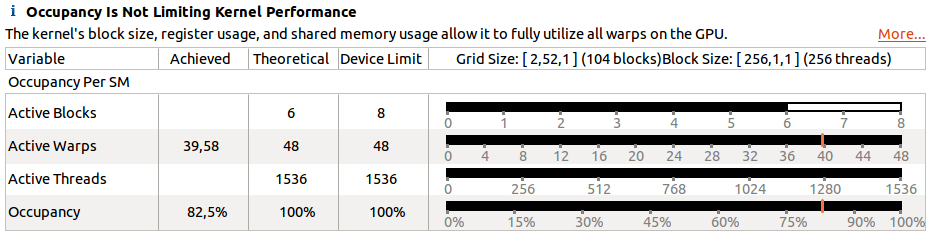
\includegraphics[width=0.7\linewidth]{profiling/darker/darker_occupancy_00}
    \caption{Img00}
    \label{fig:histo}
\end{figure}
\FloatBarrier

\begin{figure}[ht]
    \centering
    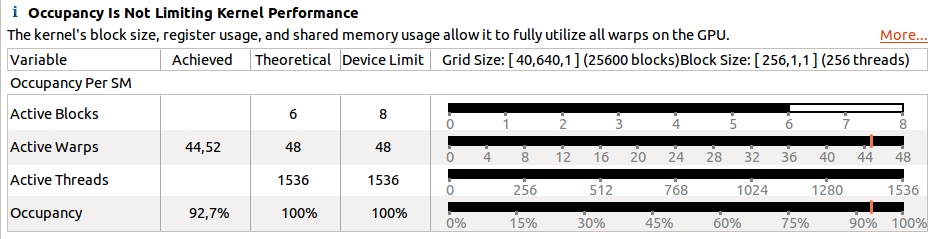
\includegraphics[width=0.7\linewidth]{profiling/darker/darker_06_occupancy}
    \caption{Img05}
    \label{fig:histo}
\end{figure}
\FloatBarrier

\begin{figure}[ht]
    \centering
    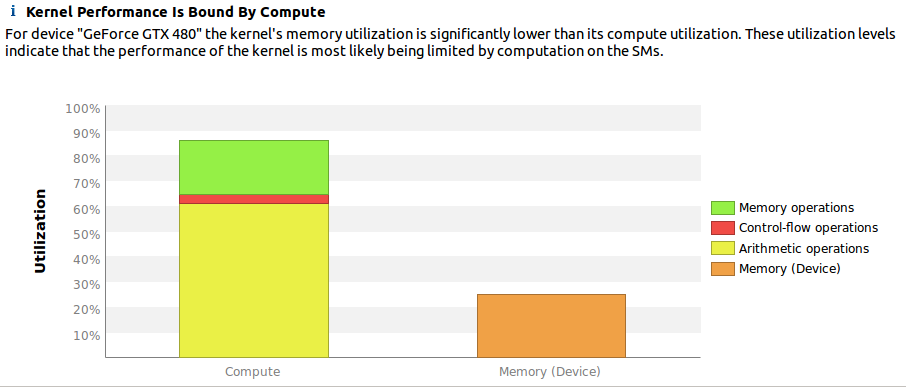
\includegraphics[width=0.7\linewidth]{profiling/darker/darker_utilization_00}
    \caption{Img05}
    \label{fig:histo}
\end{figure}
\FloatBarrier

\begin{figure}[ht]
    \centering
    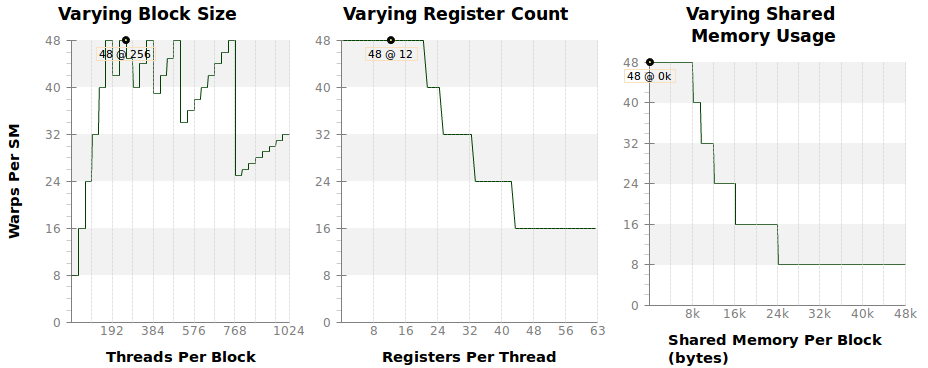
\includegraphics[width=0.7\linewidth]{profiling/darker/darker_varying}
    \caption{Img05}
    \label{fig:histo}
\end{figure}
\FloatBarrier



\begin{figure}[ht]
    \centering
    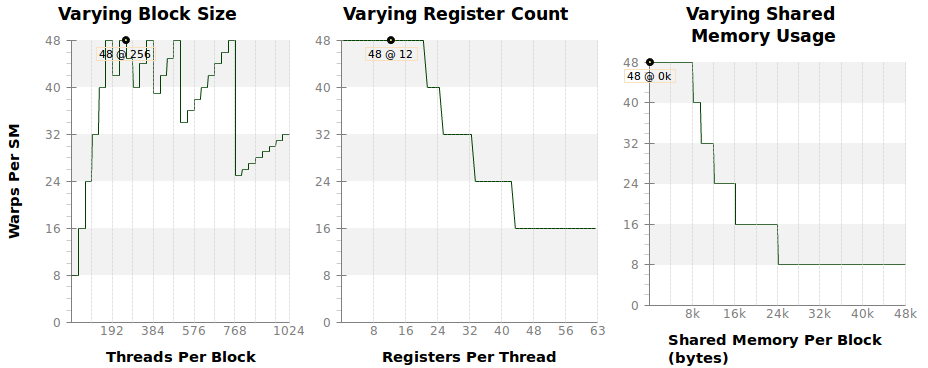
\includegraphics[width=0.7\linewidth]{profiling/darker/darker_varying}
    \caption{Img05}
    \label{fig:histo}
\end{figure}
\FloatBarrier

\printbibliography 

\end{document}

			 	 